%% bare_conf.tex
%% V1.4b
%% 2015/08/26
%% by Michael Shell
%% See:
%% http://www.michaelshell.org/
%% for current contact information.
%%
%% This is a skeleton file demonstrating the use of IEEEtran.cls
%% (requires IEEEtran.cls version 1.8b or later) with an IEEE
%% conference paper.
%%
%% Support sites:
%% http://www.michaelshell.org/tex/ieeetran/
%% http://www.ctan.org/pkg/ieeetran
%% and
%% http://www.ieee.org/

%%*************************************************************************
%% Legal Notice:
%% This code is offered as-is without any warranty either expressed or
%% implied; without even the implied warranty of MERCHANTABILITY or
%% FITNESS FOR A PARTICULAR PURPOSE! 
%% User assumes all risk.
%% In no event shall the IEEE or any contributor to this code be liable for
%% any damages or losses, including, but not limited to, incidental,
%% consequential, or any other damages, resulting from the use or misuse
%% of any information contained here.
%%
%% All comments are the opinions of their respective authors and are not
%% necessarily endorsed by the IEEE.
%%
%% This work is distributed under the LaTeX Project Public License (LPPL)
%% ( http://www.latex-project.org/ ) version 1.3, and may be freely used,
%% distributed and modified. A copy of the LPPL, version 1.3, is included
%% in the base LaTeX documentation of all distributions of LaTeX released
%% 2003/12/01 or later.
%% Retain all contribution notices and credits.
%% ** Modified files should be clearly indicated as such, including  **
%% ** renaming them and changing author support contact information. **
%%*************************************************************************


% *** Authors should verify (and, if needed, correct) their LaTeX system  ***
% *** with the testflow diagnostic prior to trusting their LaTeX platform ***
% *** with production work. The IEEE's font choices and paper sizes can   ***
% *** trigger bugs that do not appear when using other class files.       ***                          ***
% The testflow support page is at:
% http://www.michaelshell.org/tex/testflow/



\documentclass[a4, conference]{IEEEtran}
\IEEEoverridecommandlockouts
% \usepackage{graphicx}
% \usepackage{cite}
% \usepackage{amsmath,amssymb,amsfonts}
% \usepackage{algorithmic}

\def\BibTeX{{\rm B\kern-.05em{\sc i\kern-.025em b}\kern-.08em
    T\kern-.1667em\lower.7ex\hbox{E}\kern-.125emX}}

%make sure in A4 paper
\usepackage[left=1.57cm,right=1.57cm,top=0.95cm,bottom=2.54cm]{geometry}
\usepackage{graphicx}

% correct bad hyphenation here
\hyphenation{op-tical net-works semi-conduc-tor}


\begin{document}
\bstctlcite{IEEEexample:BSTcontrol}
%
% paper title
% Titles are generally capitalized except for words such as a, an, and, as,
% at, but, by, for, in, nor, of, on, or, the, to and up, which are usually
% not capitalized unless they are the first or last word of the title.
% Linebreaks \\ can be used within to get better formatting as desired.
% Do not put math or special symbols in the title.
\title{LLM-Driven CIDOC-CRM Knowledge Graph Extraction from Museum Archives}

%\author{\small *No authors informations during review process.}
% author names and affiliations
% use a multiple column layout for up to three different
% affiliations
% \author{\IEEEauthorblockN{Michael Shell}
%     \IEEEauthorblockA{School of Electrical and\\Computer Engineering\\
%         Georgia Institute of Technology\\
%         Atlanta, Georgia 30332--0250\\
%         Email: http://www.michaelshell.org/contact.html}
%     \and
%     \IEEEauthorblockN{Homer Simpson}
%     \IEEEauthorblockA{Twentieth Century Fox\\
%         Springfield, USA\\
%         Email: homer@thesimpsons.com}
%     \and
%     \IEEEauthorblockN{James Kirk\\ and Montgomery Scott}
%     \IEEEauthorblockA{Starfleet Academy\\
%         San Francisco, California 96678--2391\\
%         Telephone: (800) 555--1212\\
%         Fax: (888) 555--1212}}

% conference papers do not typically use \thanks and this command
% is locked out in conference mode. If really needed, such as for
% the acknowledgment of grants, issue a \IEEEoverridecommandlockouts
% after \documentclass

% for over three affiliations, or if they all won't fit within the width
% of the page, use this alternative format:
% 
%\author{\IEEEauthorblockN{Michael Shell\IEEEauthorrefmark{1},
%Homer Simpson\IEEEauthorrefmark{2},
%James Kirk\IEEEauthorrefmark{3}, 
%Montgomery Scott\IEEEauthorrefmark{3} and
%Eldon Tyrell\IEEEauthorrefmark{4}}
%\IEEEauthorblockA{\IEEEauthorrefmark{1}School of Electrical and Computer Engineering\\
%Georgia Institute of Technology,
%Atlanta, Georgia 30332--0250\\ Email: see http://www.michaelshell.org/contact.html}
%\IEEEauthorblockA{\IEEEauthorrefmark{2}Twentieth Century Fox, Springfield, USA\\
%Email: homer@thesimpsons.com}
%\IEEEauthorblockA{\IEEEauthorrefmark{3}Starfleet Academy, San Francisco, California 96678-2391\\
%Telephone: (800) 555--1212, Fax: (888) 555--1212}
%\IEEEauthorblockA{\IEEEauthorrefmark{4}Tyrell Inc., 123 Replicant Street, Los Angeles, California 90210--4321}}




% use for special paper notices
%\IEEEspecialpapernotice{(Invited Paper)}




% make the title area
\maketitle

% As a general rule, do not put math, special symbols or citations
% in the abstract
\begin{abstract}
    Museum archives contain vast amounts of cultural heritage information, but accessing, integrating and analyzing this data effectively remains challenging. Knowledge graphs (KGs), particularly those structured according to ontologies such as the CIDOC Conceptual Reference Model (CIDOC-CRM), offer a powerful solution through semantic representation, facilitating complex queries across diverse datasets. However, traditional KG construction is labor-intensive. Recent advancements in Large Language Models (LLMs) present an opportunity for automated knowledge extraction. This paper investigates the feasibility and effectiveness of using LLMs for constructing CIDOC-CRM knowledge graphs from museum archives, employing a single-stage in-context learning approach guided by a derived ontology. We present a case study using the online archives of the Museum Nasional in Jakarta, Indonesia. The constructed knowledge graphs are evaluated using both intrinsic (ontology conformance) and extrinsic (Knowledge Base Question Answering - KBQA) metrics.

    Evaluation results show that larger models (e.g., DeepSeek R1) are capable of high ontology conformance (up to 98.73\%) while smaller models struggle to reach 50\% conformance. While all generated KGs improved KBQA performance over a no-context baseline, the ontology-guided approach showed limited and mixed impact on KBQA accuracy compared to the ontology-free graphs in our setup. This research underscores the potential of LLMs for generating ontology-conformant KGs within the cultural heritage domain and highlights the need for more sophisticated evaluation benchmarks to assess CIDOC-CRM KG generation methods.
\end{abstract}

% no keywords

% For peer review papers, you can put extra information on the cover
% page as needed:
% \ifCLASSOPTIONpeerreview
% \begin{center} \bfseries EDICS Category: 3-BBND \end{center}
% \fi
%
% For peerreview papers, this IEEEtran command inserts a page break and
% creates the second title. It will be ignored for other modes.
\IEEEpeerreviewmaketitle



\section{Introduction}
\label{sec:introduction}

The increasing volume of information within cultural heritage institutions, such as museum archives, presents significant challenges for effective knowledge management and access \cite{alexiev2018museum}. Knowledge graphs (KGs) offer a powerful solution by representing entities and their relationships in a structured and machine-readable format, enabling advanced functionalities like semantic search, data integration, and reasoning \cite{hofer2024constructionofknowledge}. These structured representations are crucial for unlocking the potential of cultural heritage data and facilitating its wider use. Initiatives such as Linked Open Data (LOD) exemplify the application of knowledge graph principles to enhance data integration and interoperability across cultural heritage institutions \cite{pedro2013connectingthesmithsonian,dutia2021heritageconnector}. These efforts often leverage ontologies such as the CIDOC Conceptual Reference Model \cite{doerr2005thecidoc} (CRM) to provide a shared framework for describing cultural objects, events, and their interrelationships, facilitating interoperability and data sharing across institutions.

Traditionally, the construction of ontology-conformant KGs is a labor-intensive process requiring expert knowledge in both the domain and the ontology \cite{hofer2024constructionofknowledge}. However, the recent advancements in Large Language Models (LLMs) have demonstrated remarkable in-context learning abilities, allowing them to generalize over a wide range of language tasks, including complex information extraction \cite{remadi2024topromptornottoprompt}, without the need for expensive fine-tuning. This opens up new possibilities for automated knowledge extraction and KG construction \cite{ibrahim2024asurveyonaugmentingknowledgegraphs,zhu2024llmsknowledgegraphconstruction}, and in this case specifically, processing unstructured textual data from museum archives and mapping the extracted information to the concepts and relationships defined in ontologies like the CIDOC-CRM \cite{bruseker2017culturalheritagedatamanagement}.

This paper investigates the feasibility and effectiveness of using LLMs to construct CIDOC-CRM knowledge graphs from museum archives. We present a case study using the online archives of the Museum Nasional in Jakarta, Indonesia, where we construct a textual dataset from web pages dedicated to specific collections or exhibits, then employ an in-context learning approach to extract knowledge graph triplets according to a CIDOC-CRM-derived ontology. A key aspect of our approach is the integration of this ontology directly within a single-stage prompting process, with our hypothesis being knowledge graphs that are semantically richer and more accurate.

To evaluate the constructed knowledge graphs, we employ both an intrinsic and extrinsic evaluation method. The intrinsic evaluation measures the conformance of the generated graphs to the CIDOC-CRM ontology. The extrinsic evaluation is conducted through a Knowledge Base Question Answering (KBQA) task, where we use the knowledge graph as context for an LLM to answer questions related to the museum collections. This study aims to contribute to the growing body of research on leveraging LLMs and ontologies for knowledge graph generation, specifically in the cultural heritage domain, with the motivation of improving the interoperability and accessibility of cultural heritage information across institutions.

\section{Related Work}
\label{sec:related_work}

\subsection{Cultural Heritage Ontologies and Semantic Web}

In computer science, ontologies serve as formal, explicit specifications of a shared conceptualization for a domain of interest. They define the relevant classes (concepts), properties (attributes), and relationships between entities, along with axioms constraining their interpretation. Ontologies provide the semantic schema or backbone for Knowledge Graphs (KGs), which represent entities and their connections as nodes and edges.

The CIDOC Conceptual Reference Model \cite{doerr2005thecidoc} (CIDOC-CRM, ISO 21127) is a major foundation ontology designed for the integration of cultural heritage information. Its event-centric modeling paradigm, which structures information around events linking actors, objects, places, and times, captures the rich contextual history crucial for understanding cultural objects and collections. Consequently, CIDOC-CRM serves as a vital tool for structuring knowledge extracted from diverse sources, including museum archives, and building interoperable cultural heritage knowledge graphs.

\subsection{Ontology-Guided Knowledge Graph Generation}

Ontology-guided knowledge graph generation focuses on leveraging formal ontologies to guide the extraction of structured knowledge from unstructured or semi-structured text. By providing a predefined schema of concepts and relationships, ontologies ensure that the generated knowledge graphs are semantically consistent, well-structured, and aligned with a specific domain \cite{hofer2024constructionofknowledge}.

Several recent studies have explored the use of Large Language Models (LLMs) for knowledge graph generation. Xu et al \cite{xu2024chattf} utilize a two-stage prompting method guided by an ontology derived from CIDOC-CRM to extract knowledge graph triplets from textual data about Chinese traditional folklore. Beyond the cultural heritage domain, Van Cauter and Yakovets \cite{cauter2024ontology} demonstrate KG generation from maintenance short texts, while Carriero et al \cite{carriero2025humanevaluationofprocedural} construct KGs from procedural texts such as recipes or manuals. These studies often experiment with different prompting strategies to optimize the extraction process. In particular, Iga et al \cite{iga2024assessllm} demonstrate the impact of well-crafted prompts, specifically those employing in-context learning and chain-of-thought techniques, in yielding significant improvements. This highlights the importance of effective prompting methodologies to guide LLMs to generate accurate and consistent knowledge graphs aligned with a given ontology.

Our research focuses on the extraction of knowledge graphs from museum archives using an ontology derived from the CIDOC-CRM. Unlike the two-stage prompting approach employed by \cite{xu2024chattf}, we explore the effectiveness of a single-stage prompting method. Moreover, our study incorporates a comprehensive evaluation strategy that includes both intrinsic (ontology conformance) and extrinsic (KBQA task) metrics.

\section{Methods}
\label{sec:methods}

The methodology consists of the following key steps: ontology and dataset construction, knowledge graph generation (ontology-driven and ontology-free), and knowledge graph evaluation (intrinsic and extrinsic).

\subsection{Ontology Construction}

This study employs the CIDOC Conceptual Reference Model (CRM) to structure the knowledge graphs extracted from cultural heritage texts. Due to the sheer size and complexity of the CIDOC-CRM, we derived a smaller ontology for use within our LLM prompting framework.

This ontology was constructed by identifying the CIDOC-CRM classes and properties most relevant to describing museum objects, their history, and cultural context based on the expected content of the source material. The selection included core entities for physical objects, actors, places, and time-spans, key events related to object lifecycle and provenance (like production, acquisition, modification), and essential descriptive concepts (such as materials, types, titles, and dimensions).

\subsection{Dataset Construction}

The museum's official public website contains a wealth of information about its collection, with many exhibits and artifacts having dedicated articles. These articles were used to construct a dataset of textual information from the museum's collection. We collected 40 such articles such that each entry of the dataset represented a complete article dedicated to a particular item.

A custom Question-Answering (QA) dataset was also created to test knowledge about the information contained within the museum archives and to evaluate whether a knowledge graph contains the expected information from the source text. The QA dataset includes 200 questions: 185 questions about individual item-specific facts, and 15 questions about comparative facts across multiple items.

\subsection{Knowledge Graph Generation}

In addition to an ontology-guided graph generation approach, we also implement an ontology-free approach in order to evaluate the impact of ontology guidance on information quality via KBQA evaluation. Both approaches utilized a single-stage prompting method. The prompts were constructed based on level 4 of the TELeR prompt taxonomy \cite{santu2023telergeneraltaxonomyllm}, consisting of a high-level goal description, a bulleted list of sub-tasks, as well as input/output examples to facilitate in-context learning.

\subsubsection{Ontology-Guided}

This approach leverages an ontology to guide the LLM in extracting structured information. The process consists of the following steps:

\begin{enumerate}
    \item Ontology Verbalization: The ontology is verbalized into a natural language description. We use the 24037 Erlangen CRM implementation of CIDOC-CRM 7.1.3.
    \item System Prompt Construction: A system prompt is constructed from the following elements:
          \begin{itemize}
              \item A clear task description instructing the LLM to extract entities and relationships from the input text and represent them as a knowledge graph adhering to the provided ontology.
              \item Examples demonstrating desired output format.
              \item The verbalized ontology, appended at the end of the system prompt.
          \end{itemize}
    \item Chat History Initialization: The chat history is initialized with an example input and output to serve as an in-context learning mechanism.
    \item Triplet Extraction: The system prompt, chat history and text chunk are sent to the LLM. The response is parsed as a JSON list of triplets.
\end{enumerate}

\subsubsection{Ontology-Free}

The ontology-free approach aims to extract general knowledge graphs without specific guidance from the CIDOC-CRM ontology. It is nearly identical to the ontology-driven approach with the following key differences:

\begin{itemize}
    \item The task description instructed the LLM to identify entities and relationships relevant to museum collections and exhibits in the input text.
    \item The example input-output pairs demonstrated the extraction of general relationships without mapping them to a specific ontology.
    \item No verbalized ontology was included in the system prompt.
\end{itemize}

This ontology-free approach serves as a comparison point within the extrinsic evaluation, specifically to measure the impact of incorporating the ontology on the graph's accuracy via KBQA performance.

\subsection{Knowledge Graph Evaluation}

To evaluate the constructed knowledge graphs, we employ both intrinsic and extrinsic evaluation methods. The intrinsic evaluation measures the conformance of the generated graphs to the CIDOC-CRM ontology. The extrinsic evaluation is conducted through a Knowledge Base Question Answering (KBQA) task, where we use the knowledge graph as context for an LLM to answer questions related to the museum collections.

\subsubsection{Intrinsic: Ontology Conformance}

This metric aims to validate that the extracted subject-predicate-object triplets are consistent with the provided ontology. Building upon the Ontology Conformance (OC) metric from Text2KGBench \cite{mihindukulasooriya2023text2kgbench}, our approach not only checks if the predicate (property) is defined in the ontology, but also verifies that the subject and object of each triplet are valid instances of the domain and range specified for that particular property within the CIDOC-CRM.

\subsubsection{Extrinsic: Knowledge Base Question Answering (KBQA) Task}

In the absence of a "ground truth" graph, we evaluated KG accuracy by conducting an extrinsic evaluation using a Knowledge Base Question Answering (KBQA) task.

This task involved a curated set of 200 factual questions derived directly from the Museum Nasional archive dataset. The question set comprised 185 "single-item" questions, each focusing on specific details within individual item descriptions, with at least one question for each artifact/item in the source archives. Additionally, 15 more complex "multi-item" questions were created which require the model to synthesize information across multiple items to arrive at the correct answer.

For each model tested, we produced two knowledge graphs: one constructed without explicit ontology guidance and another guided by our CIDOC-CRM-derived ontology. These two graphs, along with a no-context "blank" baseline, were evaluated on the KBQA task. The blank baseline involved querying the LLM directly with the questions, without providing any knowledge graph as context, serving as a control to gauge the model's inherent knowledge about the museum's collection.

The KBQA task was executed by constructing a system prompt. For the ontology-guided and ontology-free knowledge graphs, the prompt included a verbalized representation of the respective graph as the primary context, instructing the LLM to answer each multiple-choice question (with options "A", "B", "C", or "D") using only the information provided in the context. Meanwhile, the no-context baseline prompt simply presented the question to the LLM without any additional context.

The overall performance for each evaluated knowledge graph and the no-context baseline was then calculated as the percentage of questions answered correctly, resulting in a "single-item", "multi-item", and an overall accuracy score (out of 100). The final score for each question is determined by a "best-of-three" approach, requiring the LLM to answer correctly in at least two of three attempts.

This methodology allowed us to quantitatively assess the extent to which the generated knowledge graphs, particularly the ontology-guided one, enhanced the LLM's ability to accurately retrieve and reason over information from the museum archives.

\section{Experiment}
\label{sec:experiment}

\begin{table}[h]
    \centering
    \caption{Models used for Knowledge Graph Generation} % Updated caption slightly
    \label{tab:model_deployment}
    \begin{tabular}{ll}
        \hline
        Model        & Deployment         \\
        \hline
        Qwen 2.5 3B  & Ollama on RTX 3060 \\
        Llama 3.2 3B & Ollama on RTX 3060 \\
        Qwen 2.5 7B  & LM Studio          \\
        Llama 3.1 8B & LM Studio          \\
        DeepSeek V3  & DeepSeek Platform  \\
        DeepSeek R1  & DeepSeek Platform  \\
        \hline
    \end{tabular}
\end{table}


We conducted experiments involving two main stages: \textbf{knowledge graph generation} and \textbf{knowledge graph evaluation}.

For the knowledge graph generation stage, we produced two sets of graphs from the collected textual dataset: one using an ontology-free approach and one using an ontology-guided approach. This generation was performed using open-weight LLMs of various sizes, specifically Llama 3 \cite{grattafiori2024llama3herdmodels} (3B and 8B) and Qwen 2.5 \cite{qwen2025qwen25technicalreport} (3B and 7B) deployed on local hardware, and DeepSeek \cite{deepseekai2024deepseekv3technicalreport,deepseekai2025deepseekr1incentivizingreasoningcapability} models (V3 and R1) accessed via API endpoints (Table \ref{tab:model_deployment}). In total, we generated twelve knowledge graphs: an ontology-free and an ontology-guided graph for each of the six listed models.

These constructed knowledge graphs were then subjected to evaluation. The intrinsic evaluation (Ontology Conformance), as described in Section \ref{sec:methods}, was performed on the ontology-guided graphs generated by each model. For the extrinsic evaluation, the Knowledge Base Question Answering (KBQA) task was conducted. In this task, the DeepSeek V3 model, accessed via the DeepSeek Platform, was employed as the question-answering model. For each question in the curated dataset, the DeepSeek V3 model was prompted to provide an answer based on one of the following contexts:
\begin{itemize}
    \item A verbalized representation of the ontology-free knowledge graph generated by one of the six distinct models
    \item A verbalized representation of the ontology-guided knowledge graph generated by one of the six distinct models
    \item A blank context, where the DeepSeek V3 model received only the question without any generated graph information
\end{itemize}

This setup allowed us to evaluate the question-answering performance when leveraging graphs generated by different models and approaches, comparing them against each other as well as a no-context "blank" scenario.

\section{Results}

\subsection{Ontology Conformance Evaluation}

\begin{table}[h]
    \centering
    \caption{Ontology Conformance}
    \label{tab:oc_percent}
    \begin{tabular}{|l|c|c|c|}
        \hline
        Graph       & Total Triplets & Valid Triplets & Valid Triplets (\%) \\
        \hline
        Qwen 2.5 3B & 364            & 177            & 48.63               \\
        \hline
        Llama 3 3B  & 417            & 218            & 52.28               \\
        \hline
        Qwen 2.5 7B & 443            & 225            & 50.79               \\
        \hline
        Llama 3 8B  & 519            & 332            & 63.97               \\
        \hline
        DeepSeek V3 & 630            & 596            & 94.6                \\
        \hline
        DeepSeek R1 & 630            & 622            & \textbf{98.73}      \\
        \hline
    \end{tabular}
\end{table}

\begin{figure}[!t]
    \centering
    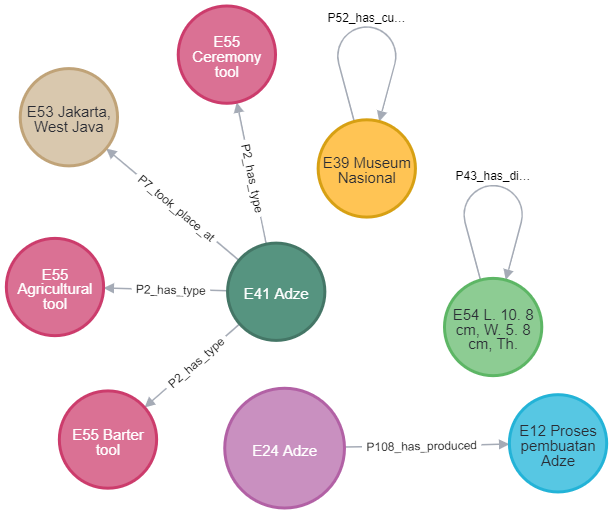
\includegraphics[width=3in]{assets/graph-qwen3b-adze}
    \caption{Ontology-guided graph from text "Adze" - Qwen2.5 3B}
    \label{fig_graph_qwen3b_adze}
\end{figure}

\begin{figure}[!t]
    \centering
    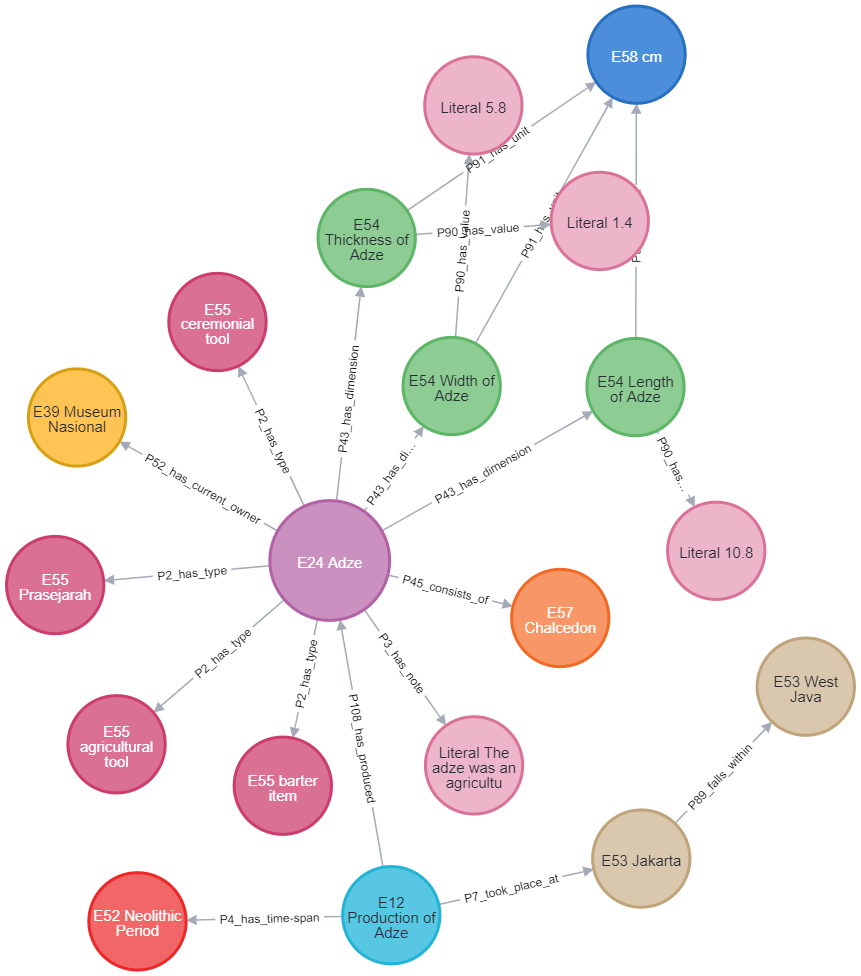
\includegraphics[width=3in]{assets/graph-r1-adze}
    \caption{Ontology-guided graph from text "Adze" - DeepSeek R1}
    \label{fig_graph_r1_adze}
\end{figure}

Table \ref{tab:oc_percent} presents the ontology conformance scores for the knowledge graphs generated by the LLMs. Achieving high ontology conformance is a fundamental requirement for any viable method aiming to construct CIDOC-CRM knowledge graphs, as a knowledge graph that does not adhere to the ontology's specifications lacks the semantic consistency necessary for downstream use cases.

The results clearly illustrate a positive correlation between the parameter size of the language model and the resulting ontology conformance. Smaller models, such as Qwen 2.5 3B (48.63\%) and Llama 3 3B (52.28\%) performed with considerably low conformance rates, while increasing the parameter count led to improvements as seen with Qwen 2.5 7B (50.79\%) and Llama 3 8B (63.97\%). Figures \ref{fig_graph_qwen3b_adze} and \ref{fig_graph_r1_adze} visually demonstrate this difference, showing example triplets extracted from the same source text about "Adze"\footnote{https://www.museumnasional.or.id/604/}.

However, a significant performance gap exists between these smaller models and the larger DeepSeek models. DeepSeek V3 achieved a high score of 94.6\%, and DeepSeek R1 reached an impressive \textbf{98.73\%} ontology conformance. This suggests that accurately interpreting and applying ontology constraints remains a considerably more challenging task for smaller language models compared to their larger counterparts.

\subsection{KBQA Evaluation}

\begin{table}[h]
    \centering
    \caption{KBQA score (overall)}
    \label{tab:qa_percent}
    \begin{tabular}{|l|c|c|r|}
        \hline
        Graph       & Ontology-Free               & Ontology-Guided & Impact \\
        \hline
        Blank       & \multicolumn{2}{|c|}{60.50} &                          \\
        \hline
        Qwen 2.5 3B & 73.50                       & 68.50           & -5.00  \\
        \hline
        Llama 3 3B  & 79.50                       & 78.00           & -1.50  \\
        \hline
        Qwen 2.5 7B & 95.50                       & 87.50           & -8.00  \\
        \hline
        Llama 3 8B  & 92.00                       & 90.50           & -1.50  \\
        \hline
        DeepSeek V3 & \textbf{98.00}              & \textbf{97.50}  & -0.50  \\
        \hline
        DeepSeek R1 & 97.50                       & 95.00           & -2.50  \\
        \hline
    \end{tabular}
\end{table}

\begin{table}[h]
    \centering
    \caption{KBQA score (single item)}
    \label{tab:qa_percent_single}
    \begin{tabular}{|l|c|c|r|}
        \hline
        Graph       & Ontology-Free               & Ontology-Guided & Impact \\
        \hline
        Blank       & \multicolumn{2}{|c|}{62.16} &                          \\
        \hline
        Qwen 2.5 3B & 72.97                       & 67.57           & -5.40  \\
        \hline
        Llama 3 3B  & 80.54                       & 78.92           & -1.62  \\
        \hline
        Qwen 2.5 7B & 95.68                       & 89.19           & -6.49  \\
        \hline
        Llama 3 8B  & 94.05                       & 91.89           & -2.16  \\
        \hline
        DeepSeek V3 & \textbf{100.00}             & \textbf{98.38}  & -1.62  \\
        \hline
        DeepSeek R1 & 98.92                       & 96.22           & -2.70  \\
        \hline
    \end{tabular}
\end{table}

\begin{table}[h]
    \centering
    \caption{KBQA score (multi item)}
    \label{tab:qa_percent_multi}
    \begin{tabular}{|l|c|c|r|}
        \hline
        Graph       & Ontology-Free            & Ontology-Guided & Impact \\
        \hline
        Blank       & \multicolumn{2}{|c|}{40} &                          \\
        \hline
        Qwen 2.5 3B & 80.00                    & 80.00           & 0.00   \\
        \hline
        Llama 3 3B  & 66.67                    & 66.67           & 0.00   \\
        \hline
        Qwen 2.5 7B & \textbf{93.33}           & 66.67           & -26.66 \\
        \hline
        Llama 3 8B  & 66.67                    & 73.33           & 6.66   \\
        \hline
        DeepSeek V3 & 73.33                    & \textbf{86.67}  & 13.34  \\
        \hline
        DeepSeek R1 & 80.00                    & 80.00           & 0.00   \\
        \hline
    \end{tabular}
\end{table}

The results of the Knowledge Base Question Answering (KBQA) task, designed to evaluate the practical utility of the generated knowledge graphs, are presented in Tables \ref{tab:qa_percent}, \ref{tab:qa_percent_single}, and \ref{tab:qa_percent_multi}. These tables report the overall accuracy (n=200), the accuracy on single-item questions (n=185), and the accuracy on multi-item questions (n=15), respectively, for both ontology-free and ontology-guided knowledge graphs generated by each tested LLM, in addition to the no-context "blank" test. Providing any graph as context significantly improved QA performance over the blank baseline, confirming the value of extracted knowledge. The blank baseline's reasonable performance, especially on single-item questions, suggests the evaluator model (DeepSeek V3) possesses some inherent knowledge related to the domain.

Consistent with the ontology conformance results, larger models generally produced graphs that lead to better KBQA scores, although the performance gap between models was less pronounced here than in the conformance task. This indicates that even models struggling with strict ontology adherence can still extract useful factual information.

Comparing the generation approaches, ontology-free graphs surprisingly led to slightly better or equal overall and single-item KBQA performance across all models. This suggests that for retrieving specific facts, the added structure of the ontology-guided graphs did not translate into improved accuracy in this setup, and may have even slightly hindered it in some cases.

The results for multi-item questions in particular were more varied. Some models benefited from ontology guidance, while others performed worse or showed no difference. However, conclusions drawn from this subset should be cautious due to the small number of multi-item questions (n=15). A larger, more diverse set of complex questions would be needed to reliably assess the impact of ontology guidance on reasoning across the graph.

Overall, the KBQA results show that LLM-generated graphs enhance question answering, and larger models tend to perform better. However, no benefit from ontology guidance during generation for KBQA performance was consistently observed, and requires further investigation with a larger and more refined set of questions.

\section{Conclusion}

This paper explored the use of Large Language Models for automatically constructing knowledge graphs from museum archives, focusing on the CIDOC-CRM ontology. Our case study, conducted on the Museum Nasional in Jakarta's online archives, demonstrated the feasibility of a single-stage prompting approach for extracting structured information as knowledge graph triplets.

Our findings indicate a disparity in LLM capabilities: while smaller models can extract factual information, adhering to the complex constraints of the CIDOC-CRM ontology is only achievable by larger models. This highlights the enhanced capacity of larger LLMs for accurate ontological interpretation and application. Ultimately, this research underscores the significant potential of LLMs to generate meaningful, ontology-conformant knowledge graphs, offering a promising route for cultural heritage institutions to improve data management and access.

The practical value of the generated knowledge graphs was evaluated through a Knowledge Base Question Answering task. Interestingly, LLMs exhibited surprisingly strong baseline performance without the generated graphs, suggesting pre-existing knowledge of the museum's collections. While larger models showed improved KBQA accuracy, the impact of ontology guidance on this task was limited. This suggests that while crucial for semantic validity, ontology integration didn't significantly hinder factual information extraction in this evaluation. This also emphasizes the growing need for more sophisticated benchmarks that can better assess the quality of CIDOC-CRM knowledge graphs.

Our study contributes to the growing field exploring the synergy between LLMs, ontologies, and knowledge graphs within the cultural heritage domain. Our results demonstrate the potential for creating structurally sound and accurate CIDOC-CRM knowledge graphs automatically. However, we still notice much room for improvement in how we evaluate CIDOC-CRM knowledge graph generation methods, particularly in areas beyond the metrics measured in this study, such as entity duplication - the same item appearing twice in the same graph under different names. Future research could also explore other ontology integration techniques, refine datasets, and evaluate the scalability of these approaches across diverse archives. The overarching aim is to leverage these technologies to enhance cultural heritage data management, accessibility, and research.

\bibliographystyle{IEEEtran}
\bibliography{IEEEabrv,References}

% that's all folks
\end{document}
